\documentclass[tikz]{standalone}

\usepackage{kotex} 
\usepackage[english]{babel}
\usepackage{tikz}
\usepackage{textcomp}

\definecolor{sasaki}{HTML}{EF9AAF}
\definecolor{gibara}{HTML}{FFBE5C}
\definecolor{warabeda}{HTML}{E34E4F}
\definecolor{roa}{HTML}{D8368D}
\definecolor{toko}{HTML}{9D3757}
\definecolor{debiru}{HTML}{444C7D}

\begin{document}
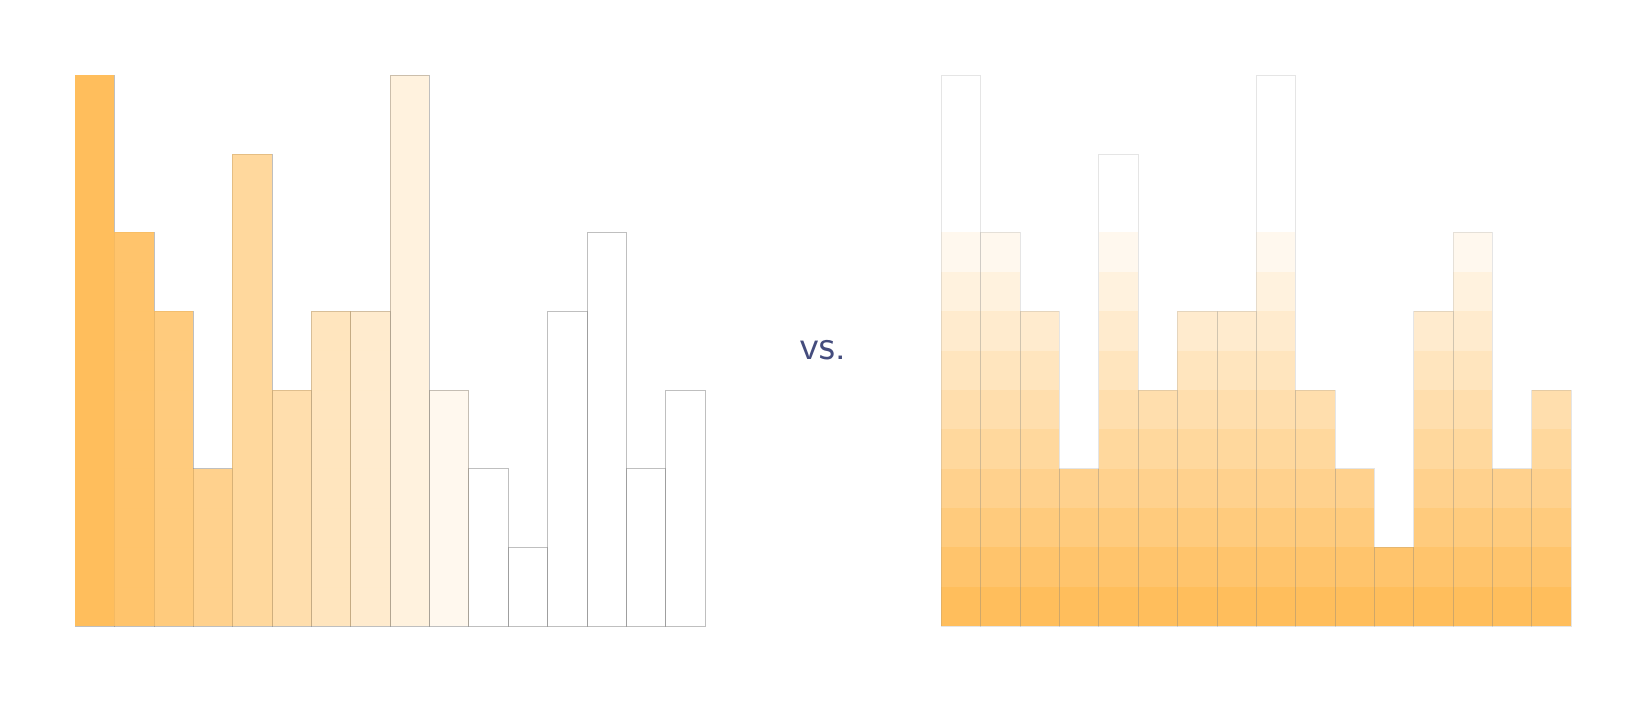
\begin{tikzpicture}
    \clip (-10.1, -.6) rectangle (10.1, 7.6);


    \draw[step=.5cm,white,ultra thin] (-10.1, -10.1) grid (10.1, 10.1);
    
    % \foreach \x in {-10, -9, ..., 10}
    %     \draw (\x, 0) node[debiru] {\textsf{\x}};
    
    % left
    \foreach \x / \y in {-9.5/7, -9/5,  -8.5/4, -8/2, -7.5/6, -7/3, -6.5/4, -6/4, -5.5/7, -5/3, -4.5/2, -4/1, -3.5/4, -3/5, -2.5/2, -2/3}
        \draw[draw=gray, ultra thin, opacity=0.5] (\x, \y) rectangle (\x+0.5, 0);
        
    \foreach \x / \y / \op in {-9.5/7/1, -9/5/0.9,  -8.5/4/0.8, -8/2/0.7, -7.5/6/0.6, -7/3/0.5, -6.5/4/0.4, -6/4/0.3, -5.5/7/0.2, -5/3/0.1}
        \draw[draw=gray, ultra thin, fill=gibara, opacity=0, fill opacity=\op] (\x, \y) rectangle (\x+0.5, 0);
    
    % right
    \foreach \y / \op in {0/1, 0.5/0.9, 1/0.8, 1.5/0.7, 2/0.6, 2.5/0.5, 3/0.4, 3.5/0.3, 4/0.2, 4.5/0.1}
        \draw[draw=gray, ultra thin, fill=gibara, opacity=0, fill opacity=\op] (1.5, \y) rectangle (9.5, \y+.5);
    
    \foreach \x / \y in {1.5/7, 2/5,  2.5/4, 3/2, 3.5/6, 4/3, 4.5/4, 5/4, 5.5/7, 6/3, 6.5/2, 7/1, 7.5/4, 8/5, 8.5/2, 9/3}
        \draw[draw=gray, ultra thin, fill=white, opacity=0, fill opacity=1] (\x, 7) rectangle (\x+0.5, \y);
    
    \foreach \x / \y in {1.5/7, 2/5,  2.5/4, 3/2, 3.5/6, 4/3, 4.5/4, 5/4, 5.5/7, 6/3, 6.5/2, 7/1, 7.5/4, 8/5, 8.5/2, 9/3}
        \draw[draw=gray, ultra thin, opacity=0.2] (\x, \y) rectangle (\x+0.5, 0);
    
    % middle
    \draw (0, 3.5) node[debiru, scale=1.5] {\textsf{vs.}};
    
    
\end{tikzpicture}
\end{document}
